\chapter[L'émergence du traitement d'images historiques]{Le traitement et l'analyse automatique de documents : comment s'est construit l'écosystème technique puis scientifique actuel.}


\lettrine{L}{'image}, à l'instar d'un document sonore ou d'une œuvre plastique, est par essence silencieuse : elle ne s'exprime que par sa propre matérialité. Aucune description, aussi minutieuse soit-elle, ne saurait véritablement se substituer à son appréhension visuelle. Pourtant, la nécessité de décrire, d'indexer et de classer ces documents non textuels s'est imposée aux professionnels du patrimoine (bibliothécaires, archivistes) bien avant l'ère des catalogues informatiques et des instruments de recherche numériques. Face à ce défi descriptif, l'idée de traiter automatiquement une image par l'analyse de ses seules caractéristiques intrinsèques, sans recourir à des métadonnées externes, est dès les origines l'une des quêtes principale de la recherche en vision artificielle\footnote{Michael Brady, \og Intelligent Vision \fg, dans \textit{AI in the 1980s and Beyond}, éditions The MIT Press, 1989}.

\section[L'origine de la vision documentaire]{Les \gls{cnn} appliqués à la vision : une technologie ancienne}

Le domaine de la vision artificielle est aussi vaste qu'un \oe il peut être utile. Il est cependant important de connaître les tâches de base, les problématiques intrinsèques de la discipline car elles en forment les contours, et donc les limites avec lesquelles doit composer le domaine des humanités. 

\subsection{La naissance de la vision artificielle appliquée aux documents}

Très fortement lié à l'imitation des capacités cognitives humaines, l'acte de naissance du \textit{machine learning} trouve sa source dans le développement du neurone algorithmique\footnote{Warren S. McCulloch \& Walter Pitts, \og A Logical Calculus of the Ideas Immanent in Nervous Activity \fg, dans \textit{The bulletin of mathematical biophysics}, Vol 5, pp. 115–133, 1943}, puis dans les travaux d'optimisation statistique. C'est avec ce principe skeuomorphique que Kunihiko Fukushima crée en 1975 le principe des réseaux de neurones convolutifs, en s'inspirant du fonctionnement du cortex visuel. Ce principe initial sera ensuite amélioré par la technique de la \og rétro-propagation du gradient \fg, découverte plus ou moins simultanément en 1985 par au moins trois équipes différentes. 


L'une des premières applications de technologies de vision à l'analyse de documents est la reconnaissance optique de caractères manuscrits pour le domaine postal et bancaire, notamment par le modèle \textit{LeNet} mis au point par \textit{AT\&T Bell Laboratories} autour de la figure de Yann LeCun entre 1988 et 1998. Avant même les bibliothèques, les archives, et les laboratoires en sciences humaines, c'est dans les industries administratives (services postaux, banques) que la vision artificielle et l'analyse automatique de documents trouvent une première application concrète notamment dans la lecture de numéros de chèques et de codes postaux. \textit{LeNet} est également l'acte de naissance de l'apprentissage profond.

\subsection{La mise en place de la vision dans les institutions patrimoniales françaises}

L'utilisation de la vision artificielle à la \gls{bnf} se concentre d'abord sur le texte et l'\gls{ocr} notamment avec l'introduction du mode texte dans Gallica à partir de 2005 et du \textit{projet d'Analyse des résultats par \gls{ocr} des documents numérisés de la \gls{bnf}} par Kamel Ait-Mohand\footnote{Kamel Ait-Mohand, \og Techniques d'adaptation de modèles markoviens. Application à la reconnaissance de documents anciens\fg, Thèse de doctorat dirigé par Thierry Paquet , soutenance en 2011.} en 2008. Concernant le travail sur l'image historique et l'iconographie, les institutions patrimoniales se concentrent principalement sur des projets d'indexations et de correspondances de thésaurus comme en 2003 avec la mise en ligne de la base \textit{Mandragore} alors existante depuis 1989\footnote{Jean-Pierre Aniel, \og MANDRAGORE . Une base de données iconographiques sur les manuscrits de la \gls{bnf} \fg, dans \textit{Le médiéviste et l'ordinateur}, n°26-27, p. 18-20, 1992-1993}, ou en 2006 du projet \gls{stich}\footnote{\og STITCH : Semantic Interoperability to Access Cultural Heritage\fg , URL \href{https://actions-recherche.bnf.fr/bnf/anirw3.nsf/IX01/A2014000409\_stitch-semantic-interoperability-to-access-cultural-heritage?opendocument\&n=1\&categorie=2006}{lien vers la page action recherche}} à la \gls{bnf}. 

\subsection{2005-2010 : la prise de conscience de l'importance des données}
La décennie 2000 est également synonyme d'un changement de paradigme grâce à deux innovations. D'abord, c'est à partir de 2005 qu'il est démontré de l'intérêt de déporter les calculs d'un \gls{cnn} du processeur à une carte graphique\footnote{Dave Steinkrau, Patrice Y. Simard, Ian Buck, \og Using GPUs for Machine Learning Algorithms \fg, dans \textit{Eighth International Conference on Document Analysis and Recognition (ICDAR)}, pp.1115-1119, 2005}. Ensuite, c'est en 2006 que Fei Fei Li, une informaticienne d'origine chinoise de l'université de Standford, théorise que l'innovation dans les modèles de vision n'est pas suffisante pour améliorer leurs performances et qu'il faut alors produire des données de meilleure qualité ; ce qu'elle met en pratique en créant le jeu de données \textit{ImageNet}\footnote{J. Deng, W. Dong, R. Socher, L. -J. Li, Kai Li and Li Fei-Fei, \og ImageNet: A large-scale hierarchical image database\fg, dans \textit{2009 IEEE Conference on Computer Vision and Pattern Recognition}, Miami, FL, USA, pp. 248-255, 2009, doi: 10.1109/CVPR.2009.5206848.} en 2009 et de sa compétition associé, l'\gls{ilsvrc} un an plus tard. C'est ce tournant de 2009, passant d'une réflexion uniquement portée sur l'architecture de l'algorithme à la prise de conscience de l'importance dans la qualité et de la méthodologie de sélection des données d'entraînement qui fait entrer la vision artificielle dans sa période de maturité technologique.

\section[La vision aujourd'hui]{La décennie 2010 : le tournant des \gls{rcnn}}

Parmi ces jeux de données publiés chaque années à l'occasion de compétition, l'un des plus importants a été le dataset \textit{PASCAL VOC}. Cette compétition de détection tenue chaque année entre 2005 et 2012 démontrait que l'architecture des réseaux convolutifs devenait plus complexe mais tout en atteignant un plateau de performance. C'est en 2013 qu'est dévoilée la première architecture de réseaux à extraction de région\footnote{R. Girshick, J. Donahue, T. Darrell et J. Malik, \og Region-Based Convolutional Networks for Accurate Object Detection and Segmentation\fg dans \textit{IEEE Transactions on Pattern Analysis and Machine Intelligence}, vol. 38, no. 1, pp. 142-158, 2016, doi: 10.1109/TPAMI.2015.2437384.} \gls{rcnn} qui a l'avantage de grandement simplifier l'architecture du modèle tout en dépassant les plafonds des anciennes itérations.


Ce sont des modèles spécialisés dans la détection de région dans des images (détection, segmentation), les rendant rapidement irremplaçables dans les utilisations appliquées aux documents historiques. Le principe d'un \gls{rcnn} c'est l'application d'un pré-traitement à l'image avant d'utiliser un \gls{cnn} classique. L'opération de pré-traitement regroupe les pixels de l'image au sein d'une représentation en graphes\footnote{Lilian Weng, \og Object Detection for Dummies Part I : Gradient Vector, HOG, and SS \fg, sur \href{https:\/\/lilianweng.github.io\/posts\/2017-10-29-object-recognition-part-1\/}{lilianweng.github.io}} puis de prédire une probabilité de présence d'un objet par rapport à un fond grâce à un algorithme nommé \textit{algorithme de recherche sélective}\footnote{Pedro F. Felzenswalb, Daniel P. Huttenlocher, \og Efficient Graph-Based Image Segmentation \fg, dans \textit{International Journal of Computer Vision}, n°59, vol 2, pp.167–181, 2004}.


    \begin{figure}
        \centering
        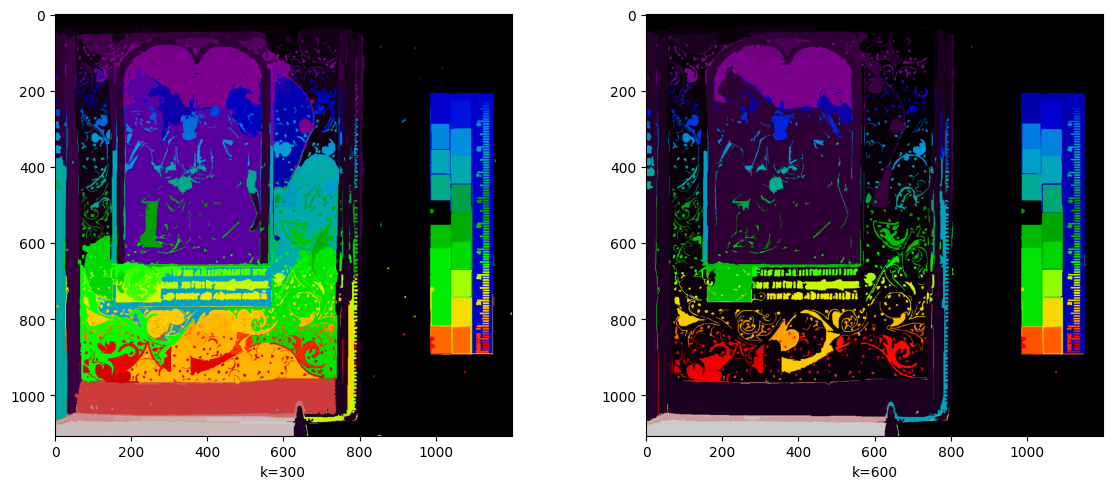
\includegraphics[scale=0.4]{img/felzenszwalb.png}
        \caption{Application d'une segmentation Felzenszwalb à une page d'un livre d'heure du dataset Horae LSv2. Premièrement avec une segmentation fine avec un seuil de tolérance bas (k=300), et un seuil de tolérance haut (k=600). Le seuil de tolérance détermine à quel point deux zones voisines doivent être différentes pour que l'algorithme refuse de les fusionner et décide de tracer une frontière entre elles.}
        \label{fig:felzenszwalb}
    \end{figure}


Rapidement, les travaux sur les modèles \gls{rcnn} vont mener à la création de sous-familles plus perfomantes comme Fast R-CNN\footnote{Ross Girshick, \og Fast R-CNN \fg, communication pour l'\textit{International Conference on  Computer Vision 2015}, 2015, URL: \href{  	
https://doi.org/10.48550/arXiv.1504.08083}{  	
https://doi.org/10.48550/arXiv.1504.08083}} pour la détection d'objets, puis Faster R-CNN qui améliore encore la performance des modèles ou Mask R-CNN qui étend les avancées de Faster R-CNN à la segmentation par pixel. 

\subsection{\textit{You Only Look Once} (\gls{yolo})}

Dans le domaine patrimonial, ces avancées se sont traduites par une meilleure performance dans la capacité des modèles à traiter des documents patrimoniaux, mais également la possibilité d'utiliser plusieurs méthodologies plus ou moins complexes. Le programme-cadre (framework) le plus populaire pour une utilisation patrimoniale est la famille des modèles \gls{yolo}  introduite par Joseph Redmon\footnote{J. Redmon, A. Farhadi, \og YOLO \fg, communication pour \textit{2016 Computer Vision and Pattern Recognition Conference}, 2016} puis amélioré à partir de la version 4 par plusieurs chercheurs, institutions et entreprises. Sa popularité tient du fait que le modèle ne fait qu'une seule proposition de région (rétro-propagation) avant d'effectuer ses prédictions, contrairement aux autres architectures de \gls{rcnn} qui peuvent répéter cette étape de rétro-propagation plusieurs milliers de fois par image. 

Les modèles de détection d'AIKON sont actuellement deux \gls{yolo} version 5\footnote{Ségolène Albouy, URL : \href{https://huggingface.co/seglinglin/Historical-Illustration-Extraction/tree/main}{sur Huggin Face}} (un pour les illustrations et un pour les diagrammes) et nous avons entraîné durant le stage un \gls{yolo} version 8 et un \gls{yolo} version 26\footnote{Jules Musquin, URL : \href{https://huggingface.co/Anarchiviste/GenHisDoc_model}{https://huggingface.co/Anarchiviste/GenHisDoc\_model}}.  AIKON utilise également d'autres types de modèles comme un Faster-RCNN pour la détection de filigranes ou la détection de lignes de texte. Aujourd'hui \gls{yolo} ne réfère plus réellement à une famille de modèles précis mais à un concept général d'architecture. Si les principaux modèles sont publiés et maintenus en open source, la bibliothèque python la plus utilisée est celle de l'entreprise \textit{Ultralytics}, critiquée pour sa tendance à s'approprier le projet \gls{yolo} qui était à la base open-source. \textit{Tiamat}, un projet similaire relativement similaire à AIKON, porté par le consortium \textit{HN-Humanum Pictoria} utilise également cette architecture \gls{yolo}\footnote{Fantin Le Ber \og IA et patrimoine, un changement dans la continuité : l’exemple du projet Highvision\fg, mémoire de master, \textit{École nationale des chartes}, 2025}. 


\subsection{\gls{detr} : le concurrent direct de \gls{yolo}}

En 2020, l'entreprise Facebook, aujourd'hui renommée Meta, dévoile l'architecture \gls{detr} qui combine une base convolutive \gls{resnet} avec un \textit{transformer} (attention globale). Si les architectures \gls{detr} ne sont pas encore énormément utilisées en production dans les institutions patrimoniales, ces modèles récupère des parts de marché. Cette avantage grandit pour deux raisons principales : 
\begin{description}
    \item \textbf{La licence d'exploitation} : La licence des modèles \gls{yolo} publiés par \textit{Ultralytics} est au format \gls{agpl}-3.0. L'utilisation est donc gratuite seulement si le projet est lui-même open-source ou l'institution doit payer une licence d'entreprise. Les modèles \gls{detr} et les environnements fournis par Meta sont aujourd'hui au format de licence Apache 2.0, autorisant une réutilisation privée ou commerciale gratuite.

    \item \textbf{Les gains de performance grầce à l'utilisation des \textit{transformers}} : \gls{detr} introduit dans la vision artificielle l'utilisation de la technologie \textit{transformers}\footnote{Ashish Vaswani, Noam Shazeer, Niki Parmar, Jakob Uszkoreit, Llion Jones, Aidan N. Gomez, Lukasz Kaiser, Illia Polosukhin, \og Attention is All You Need \fg, communication pour \textit{2017 Advances in Neural Information Processing Systems} (NIPS), 2017}. L'avantage principale de cette architecture étant l'efficacité de la parallélisation des calcules car un transformer ne demande pas un calcul séquentiel des données contrairement à un \gls{cnn}.  Dans cette nouvelle architecture, la détection de classes dans une image devient un opération d'ensemble directe (\textit{direct set prediction})\footnote{Nicolas Carion, Francisco Massa, Gabriel Synnaeve, Nicolas Usunier,
    Alexander Kirillov, Sergey Zagoruyko, \og End-to-End Object Detection with Transformers \fg, communication pour \textit{2020 European Conference on Computer Vision} (ECCV), 2020, DOI: \href{arXiv:2005.12872}{arXiv:2005.12872}}. Le programme utilise d'abord un \gls{cnn} qui permet d'extraire certaines informations de l'image, puis un couple encodeur-décodeur permettant d'extraire une prédiction pour les classes et une prédiction pour les boundings boxes\footnote{Yu Liang, Tang Lin, Mu Lisha, \og A Review of DEtection TRansformer: From Basic Architecture to Advanced Developments and Visual Perception Applications\fg, dans \textit{Sensors}, n°25, vol°13, 2025, DOI: \href{10.3390/s25133952}{10.3390/s25133952}}.
\end{description}

\section[2020 : les nouvelles approches]{La décennie 2020 : la maturité opérationnelle et l'apparition de nouvelles approches}. 

Dans le domaine de la vision, jusqu'aux \gls{rcnn} et \gls{yolo}, la détection n'était que géométrique : le modèle isolait des pixels (une boîte ou un masque) comme faisant partie d'une classe. Les chercheurs dès 2015 créent les premiers modèles de vision multimodaux combinant texte et image (\textit{image captioning systems}), ce sont des \gls{cnn} capable de générer des annotations au niveau de l'image\footnote{Kelvin Xu, Jimmy Ba, Ryan Kiros, Kyunghyun Cho, Aaron Courville, Ruslan Salakhutdinov, Richard Zemel, Yoshua Bengio, \og Show, Attend and Tell: Neural Image Caption Generation with Visual Attention\fg, publié sur ArXiv, DOI : \href{10.48550/arXiv.1502.03044}{10.48550/arXiv.1502.03044}}, et donc de faciliter les tâches de classifications. 

\subsection{Les \textit{Visual Language Models} (\gls{vlm}) : Du pixel à la sémantique}

À partir de 2018, cette approche multimodale va connaître une évolution rapide avec dans un premier temps l'application de la technologie des \textit{Transformers} qui sont fait pour le traitement du langage naturel et donc qui offrent des liens entre le texte et l'image bien plus profonds. Le domaine profite également de la création de nouveaux jeux de données d'entraînement généralisés comme \textit{MS COCO}\footnote{Tsung-Yi Lin,  Michael Maire, Serge Belongie, Lubomir Bourdev, Ross Girshick, James Hays, Pietro Perona, Deva Ramanan, C. Lawrence, Zitnick Piotr Dollar, \og Microsoft COCO: Common Objects in Context \fg, publié sur ArXiv, 2015, DOI: \href{arXiv:1405.0312v}{arXiv:1405.0312v}}, pourvoyant des annotations sous forme de paires d'images et de texte descriptif. Plusieurs nouveaux types de tâches apparaissent dans le sillage des évolutions comme le \gls{vqa} ou le \textit{Phrase Grounding} qui peut transformer un texte qui décrit une image en une référence spatialisée dans l'image avec des boîtes englobantes\footnote{Timothy M, \og What is Phrase Grounding \fg, post de blog sur Roboflow, 2024, URL : \href{https://blog.roboflow.com/what-is-phrase-grounding/}{Lien vers le blog}}.

En 2021, OpenIA rend public le premier modèle \gls{vlm} de fondation  avec  \textit{CLIP} (Contrastive Language–Image Pretraining). La capacité de traitement du texte d'un \gls{vlm}, et la montée en popularité des systèmes \gls{rag} fait que le milieu documentaire va rapidement s'imposer comme un sujet de choix pour l'application de ces technologies avec dès 2021 la mise à disposition par Microsoft de \textit{LayoutLM}\footnote{Yiheng Xu, Minghao Li, Lei Cui, Shaohan Huang, Furu Wei, Ming Zhou, \og LayoutLM: Pre-training of Text and Layout for Document Image Understanding \fg, communication pour \textit{26th ACM SIGKDD International Conference on Knowledge Discovery \& Data Mining}, 2020, DOI: \href{arXiv:1912.13318v5}{arXiv:1912.13318v5}},  un modèle permettant de joindre l'\gls{ocr} et la reconnaissance de mise en page dans des documents contemporains \gls{olr}. C'est cette articulation conjointe du visuel et du textuel qui ouvre une perspective inédite pour l'analyse de documents patrimoniaux en imitant l'humain en liant le contenu et le contenant\footnote{Sina Semnani, Han Zhang, Xinyan He, Merve Tekgurler, Monica Lam, \og CHURRO: Making History Readable with an Open-Weight Large Vision-Language Model for High-Accuracy, Low-Cost Historical Text Recognition\fg,}. 

Cependant il est intéressant de noté quelques limites à ces technologies que nous tirons d'un article de Maria Levchenko sur une méthodologie d'évaluation des VLM dans le contexte de la lecture de document historique\footnote{Maria Levchenko, \og Evaluating LLMs for Historical Document OCR: A Methodological Framework for Digital Humanities\fg, publié sur ArXiv, 2025, DOI : \href{arXiv:2510.06743v1}{arXiv:2510.06743v1}} que nous pouvons regrouper trois grands arguments. Premièrement, cette famille de modèle performent le mieux sur du texte imprimé Les testes entre VLM et R-CNN se font majoritairement sur des tâches d'OCR. Ces technologies performent le mieux dans des situations où d'autres technologies moins complexes performent également à un niveau acceptable. Cependant ils semblent présenter un avantage pour l'HTR, ou dans certaines conditions comme une mise en page difficile ou un document un peu trop abîmé\footnote{Seorin Kim , Julien Baudru, Wouter Ryckbosch, Hugues Bersini, Vincent Ginis, \og Early evidence of how LLMs outperform traditional systems on OCR/HTR tasks for historical records\fg, publié sur ArXiv, 2025, DOI : \href{arXiv:2501.11623v1}{arXiv:2501.11623v1}}. Ensuite, toutes les familles de modèles "génératifs" ont des comportements non-déterministes lors de différents passages d'un même document avec un même modèle\footnote{ Marie Puren, Donghan Bian, Aurélien Pellet, Julien Perez, Florian Cafiero, \og  Aligner méthode historique et RAG : transformer un
assistant conversationnel en chaîne de preuve auditable et
discutable\fg, communication pour \textit{Humanistica 2026, Association francophone des humanités numériques}, pp.1-9, 2026, DOI: \href{10.63744/G14mF7UizFzS }{10.63744/G14mF7UizFzS }}. Enfin, les VLM font partie des programmes les plus onéreux à faire tourner actuellement, que ce soit en terme de ressource machine (RAM, Calcule sur GPU, temps de calcule) ou en prix de déploiement chez un fournisseur. La question du passage d'un document dont la numérisation est potentiellement sous-droit dans un modèle qui n'est disponible que chez un fournisseur pose également une question de propriété intellectuelle.


\subsection{Les modèles fondateurs et l'apparition de l'approche \textit{Zero-shot} / \textit{Few-shot}}

Aujourd'hui, l'application de la vision par ordinateur aux sources historiques imposait aux chercheurs un véritable travail d'annotation sérielle. Les applications institutionnelles qui permettent l'utilisation de la vision pour public non technique dans le style d'Aikon permettent de mutualiser l'utilisation d'un modèle entre les utilisateurs et donc d'utiliser les outils plus complexes et entraînés sur plus de données. 

Pour entraîner un modèle à reconnaître détecter ou segmenter les éléments d'une page, il est indispensable de constituer \textit{ex nihilo} de volumineux jeux de données (des données que le modèle n'a jamais vu). Les équipes et les historien\pmm nes se voient ainsi contraint d'assumer le rôle de producteur de données, passant un temps considérable à tracer manuellement les annotations(\textit{bounding boxes}). 

L'émergence des modèles dits « fondateurs » (\textit{Foundation Models}) pourrait peut être rompre une partie de ce goulot d'étranglement. Pré-entraînés sur des volumes massifs d'images et de textes, des architectures multimodales comme \textit{Florence-2}\footnote{Bin Xiao, Haiping Wu, Weijian Xu, Xiyang Dai, Houdong Hu, Yumao Lu, Michael Zeng, Ce Liu, Lu Yuan, \og Florence-2: Advancing a Unified Representation for a Variety of Vision Tasks \fg, publié sur ArXiv, 2023, DOI: \href{https://arxiv.org/abs/2311.06242}{https://arxiv.org/abs/2311.06242}} ou les grands VLM généralistes disposent d'une représentation du monde visuel suffisante pour travailler sur un document historique sans entraînement préalable. Cette puissance leur permet dans certains cas de fonctionner selon deux modes inédits pour la vision patrimoniale : le \textit{Zero-shot}, capable d'exécuter une tâche de segmentation, de détection ou de description sans aucun entraînement préalable sur le corpus cible, et le \textit{Few-shot}, qui ne nécessite qu'un nombre très restreint d'exemples pour guider le modèle ou effectuer un réalignement léger (\textit{fine-tuning}).

Par exemple, après notre stage, nous avons notamment essayé d'aider Eva Rivière à faire tourner \textit{Florence-2} dans une tache d'annotation d'image de façade de bâtiments en  \textit{Zero-shot} de \textit{Phase Grounding}\footnote{Jules Musquin, Eva\_benchmark\_torne-h
 sur \href{https://github.com/Anarchiviste/Eva_benchmark_torne-h}{Github}} en offrant au modèle une image d'une façade et une description au format json des éléments à annoter. Si nous avons réussi à faire tourner un modèle aussi lourd sur nos équipements personnels, nous n'avons cependant pas réussi à sortir un image traitée correctement. Cette expérience rapide montre à la fois les espoirs que suscite cette capacité d'annotation zero-shot mais également les problèmes techniques de coût et de puissance de calcule de ces technologies. 

%L'idée forte : La décennie 2010 imposait à l'historien un travail de forçat : créer des datasets massifs (des milliers de bounding boxes) pour entraîner un modèle de zéro.

%Le basculement : L'arrivée des modèles pré-entraînés massifs (les Foundation Models comme Florence-2, SAM ou les grands LLM visuels) qui fonctionnent en Zero-shot (sans entraînement) ou avec très peu de données (Few-shot / Fine-tuning léger).

%yL'enjeu historique : Cela démocratise l'IA pour l'histoire. L'historien n'a plus besoin d'être un producteur industriel de données. L'acte de recherche se déplace : on passe de l'annotation de masse à l'ingénierie de la requête (le prompt) et au réglage fin sur des sources hyperspécifiques (ce que tu as fait avec GenHisDoc sur YOLO).



